\documentclass[12pt, titlepage]{article}
\usepackage[utf8]{inputenc}
\usepackage{graphicx}
\usepackage{indentfirst}
\usepackage[a4paper,width=150mm,top=25mm,bottom=25mm]{geometry}

\title{Weather App Project Plan}

\author{Kyle Chestnut, Caleb Newman, Trey Coleman, Alan Huebschen}

\begin{document}

\maketitle

\section*{Scope}

Our group created a GUI based weather application which was written in Python and uses the PyQt bindings to create a user interface. When the program is first opened, it queries an external web server to get the user’s external IP. It then takes that IP and queries a location database service to find the approximate location of the IP. This location is then fed into the openweathermap public API which returns not only the current weather but also a 5 day forecast. Both current weather and the 5 day forecast are displayed on the user interface. The user can also search for a location and display the associated weather data with their requested location.

\section*{Organization Chart}

We identified 4 different positions that would be vital to the completion of this project.  The positions would be a Project Manager, Designer, Coder and a Tester.  The description of the positions are as follows:

\begin{itemize}
    \item[Project Manager] Helps the team with staying on schedule while helping each member with roadblocks if problems arise.
    \item[Designer] Design the code as to how the program will work.
    \item[Coder] Write the code based upon what the designer(s) came up with.
    \item[Tester] Tests the code that was written.
\end{itemize}

\begin{center}
    \makebox[\textwidth]{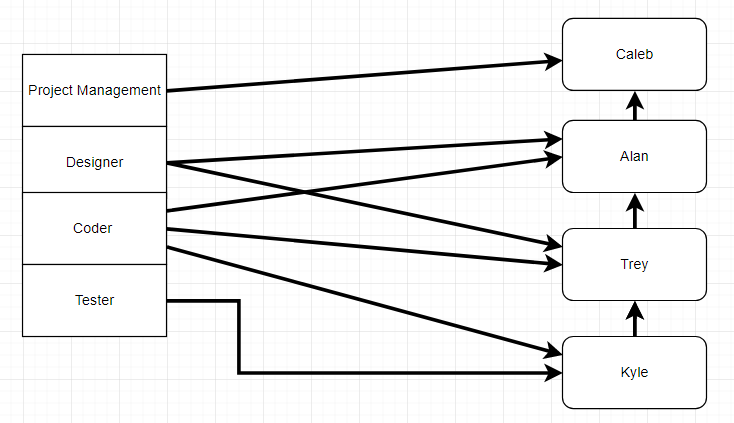
\includegraphics[width=\textwidth{...}]{org_chart.png}}
\end{center}

\pagebreak
\section*{Gantt Chart}

There were 2 major phases of our project.  The first of which was developing the current weather portion of the project.  The second of which was developing the 5 day forecast.  The steps of the phases are shown below.

\begin{center}
    \makebox[\textwidth]{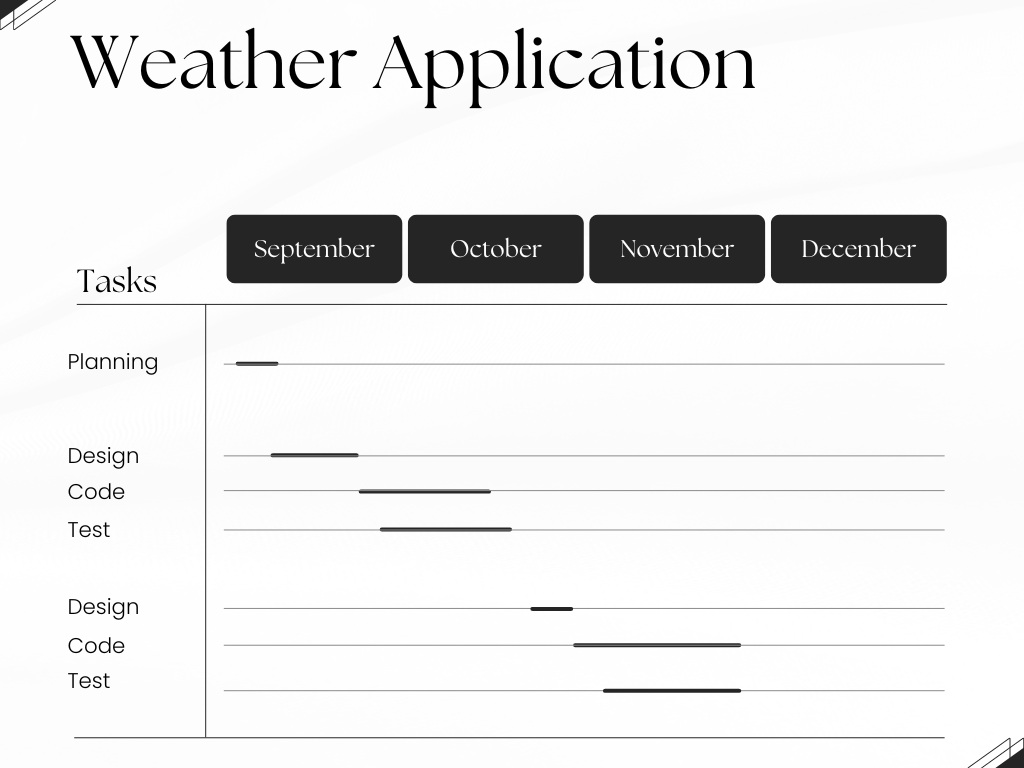
\includegraphics[width=\textwidth{...}]{gantt_chart.png}}
\end{center}

\section*{Tools and Standards}

The tools we used to complete this project were the python programming language to code the project.  Within the python programming language we used PyQt5 to build out the GUI for this project.  The integrated development environment we primarily used was Visual studio code.  To help design the look of our program we used QT designer in order to build a rough framework of where we needed each component of the user interface to be located.
As far as standards we primarily used the iterative coding standard as it would allow the coders to test early and often as working with an API was thought to come with its own set of potential issues.  The documentation standard we used follows the IEEE 830-1998 standard.

\section*{Configuration Management Plan}

We primarily used git and a private github repo with regular releases of executables as well as keeping local files of our development code versions as a backup.

\end{document}
